We can relate the polarization fraction of the radio relic to the
projection angle by examining the
generating mechanism of the radio relic.
The observed radio relic is due to synchrotron emission of free electrons in a
magnetic field. If the magnetic field is uniform, the observed
polarization fraction of the synchrotron emission of the electrons depends on the
viewing angle (or equivalently the projection angle) with respect to the alignment of the magnetic field. 
Synchrotron emission from electrons inside unorganized magnetic field are
randomly polarized. The high reported integrated polarization fraction from
\citet{L13} can be explained by a highly aligned magnetic field,
created by the compressed intracluster medium during a merger
(\citealt{E98}, \citealt{vanWeeren10}, \citealt{Feretti12}).
This picture is consistent with a high polarization fraction perpendicular
to this magnetic field along the relic. 
\par
We designed our prior to reflect how $\alpha$ decreases monotonically as the
maximum observable integrated polarization fraction. 
\begin{figure}
	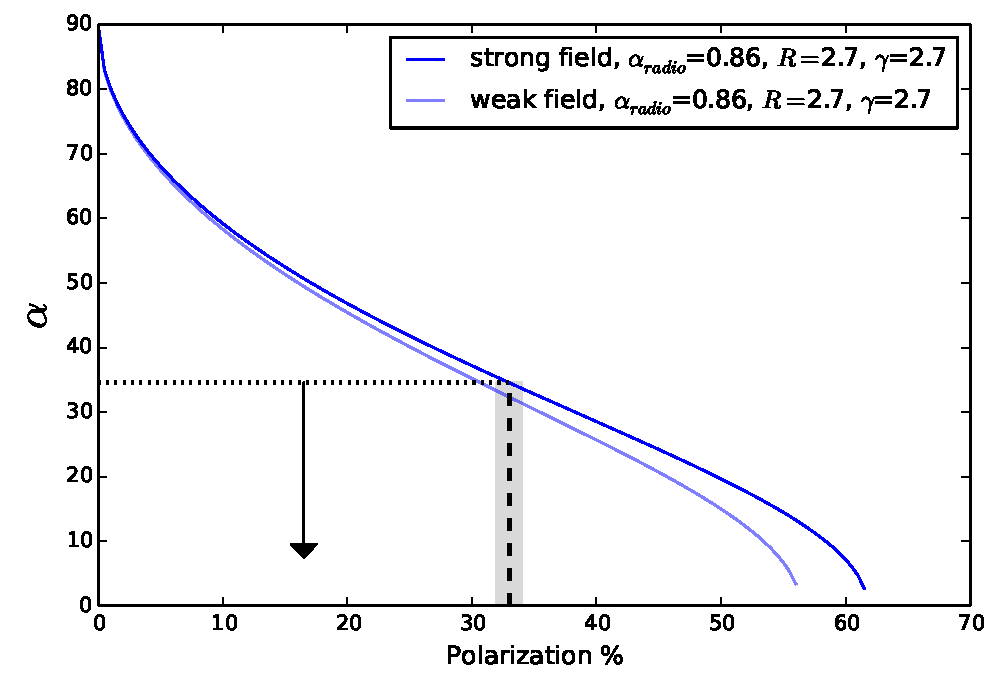
\includegraphics[width=\linewidth]{Ensslin_polar_fig.pdf}
	\caption{Predictions of polarization percentage of the radio relic at a
		given projection angle from different models, reproduced from
		\citealt{E98}. Each model assumes electrons producing the radio emission
		to be accelerated inside
		uniform magnetic field of various strengths ({\it strong} or {\it weak}). The curves are plotted with spectral index of the radio emission
		($\alpha_{radio}$), spectral index of the electrons ($\gamma$) and
		compression ratio of the magnetic field ($R$) corresponding to the
		estimated values from \citet{L13}.
		We highlight the observed polarization percentage of the main NW radio relic
		of El Gordo by the dotted vertical line with the greyed out region
		indicating the uncertainty \citep{L13}.\label{fig:Ensslin_fig}}
\end{figure}
This assumption is based on the class of models given by \cite{E98}(See
Figure~\ref{fig:Ensslin_fig}). In particular, we refer to a model from \cite{E98} that would give the most
conservative estimate on the upper bound of $\alpha$:
\begin{align}
\alpha &= 90 \degree -
\arcsin
\left(
\sqrt{
\frac{
	\frac{2}{15} \frac{13R - 7}{R - 1} \frac{\gamma + 7/3}{\gamma + 1}
	\langle P_{strong} \rangle}{
	1 + \frac{\gamma + 7/3}{ \gamma +1} \langle P_{strong} \rangle }}\right)
\end{align}


This model
corresponds to the strong field case with the relic being supported by
magnetic pressure only, with $\alpha_{radio} = 0.86$, compression ratio
$R=2.7$ and $\gamma = 2.7$. 
This model predicts a maximum integrated polarization fraction of
$\sim60\%$ when $\alpha \rightarrow 0$. From this model, the observed integrated
polarization fraction of $33\%\pm1\%$ corresponds to an estimated value
of $\hat{\alpha}
 = 35\degree$. 
%We consider 39\degree as an upper bound on the projection angle since this idealized model assume isotropic distribution of magnetic field and
%electrons. 
This  polarization fraction of $\sim 60\%$ predicted by \citep{E98} is
consistent with the upper bound of relic polarization fraction in cosmological
simulations \citep{S13}. No other model of the magnetic field should predict a higher polarization fraction, thus it is highly unlikely that we see 33\%
integrated polarization at $\alpha > 35\degree$.  
\par

We cannot rule out $\alpha \leq 35\degree$ as a result of possible
variations in the magnetic field. 
\cite{E98} assumes an isotropic distribution of electrons in an isotropic magnetic field. Cosmological
simulations of radio relics from \cite{S13} show varying polarization
fraction across and along the relic assuming $\alpha = 0$, resulting in a
lower integrated polarization fraction. For example, it is possible to see a edge-on radio relic ($\alpha = 0$) with integrated polarization fraction of 33\%. 
Furthermore, \cite{S13} shows that after convolving the
simulated polarization signal with a Gaussian kernel of 4\arcmin~to
illustrate effects of non-zero beam size, the polarization fraction drops to between 30\% to
65\% even when $\alpha = 0$. 
Other uncertainties come from the fact that the inferred spectral indices
differ between the two observed frequencies and vary between the three
identified relic sources \citep{L13}. We examine the effects  of changing
the cutoff value of this prior to ensure the uncertainties do not
introduce significant bias in the estimated output variables and we
present the results in Appendix \ref{app: results}.
To summarize, we adopt a conservative uniform prior to encapsulate the
information from the polarization fraction of the radio relic as:
\begin{equation}
P(\alpha) = 
	\begin{cases}
	& \text{const. $>$ 0 for  }\alpha < 35 \degree \\ 
	& 0 \text{ otherwise}
	\end{cases}
\end{equation}


%Due to these likely variations in the true magnetic field, the true observable integrated polarization values at a given $\alpha$ can be lower than what is predicted by \cite{E98}. 
%For example, it is possible that the radio relic of El Gordo has a lower maximum face-on polarization fraction than 75\%, but if we are viewing the relic at a smaller $\alpha$, the integrated
%polarization fraction can still comes out to be 33\%.

%With simplifying assumptions, \cite{E98} have derived the integrated polarization fraction of a radio relic as a function of the viewing
%angle ($\delta = 90\degree - \alpha$).
% and the compression
%\~{R} of the magnetized region where the relic is generated. 
%. The simplifying assumptions, such as having an
%isotropic distribution of unshocked magnetic fields and electrons etc.,
%represents an idealized case showing maximum possible polarization fraction at a given $\alpha$.  
%% Cosmological simulations of radio
%relic \citep{S13} show a maximum integrated polarization fraction $\sim75\%$ at
%$\alpha = 0$ as predicted by \cite{E98}. 
%After accounting for different spectral
%indices and magnetic field strength, 
%The simplifying
%assumptions, such as having an isotropic distribution of unshocked fields
%and an isotropic distribution of electrons etc. \citep{E98}, gives
%polarization fraction as high as $\sim$ 75\% when $\alpha = 0$. 

%For an
%actual merger, the magnetic field can be less isotropic,  and the resulting polarization fraction at a given $\alpha$ would be lower. This postulate is backed up by the edge-on view of polarization fraction of simulated relics, such as the top left hand panel of figure 9 from Skillman et al. 2013.
%%This model, however, assumes an isotropic distribution of electrons in an isotropic magnetic field. \cite{E98}
%%These mathematical relationships underlies the design of this prior based on observed polarization fraction. The different cases that \cite{E98} considered have different magnetic field strengths and various spectral indices.
%We note that power of polarized synchrotron emission from relativistic electrons has a ratio of 7:1 between parallel polarization and perpendicular polarization. 
%Therefore,   
%
%\par
%\textbf{We pick a form of uniform prior, to represent
%the uncertainties in both the modeling (\citealt{E98}, \citealt{S13}) and the interpretation of the data from \cite{L13}.} 
%Following previous discussion, we pick a value of $\mu_\alpha =39\degree +
%2 \degree$ to filter realizations, i.e. we do not draw values of $\alpha >
%41\degree$. The extra $2 \degree$ in the prior is included to account for the uncertainty of the integrated polarization fraction reported by \cite{L13}. 
%
%For the width of fall off of the sigmoidal function, we pick
%$\sigma_\alpha = 1\degree$ that corresponds to the uncertainty of the
%integrated polarization fraction reported by \cite{L13}.    

%\begin{itemize}
%\item spectral index of ...
%\item During the merger process, the hot intracluster is cluster merger compresses the magnetic field and orders the polarization.    
%\item \cite{L13} reported that the polarization can constrain viewing angle to be $> 18 \degree $-- check if this viewing angle is defined the same way 
%\item Ensslin 's work which is an application of the theory of
%plane-parallel shock acceleration, which can be justified by the large
%radius of the shock sphere
%\item we consider the most conservative constraint that can be recovered
%from this model, which is strong/weak field case with a spectral index of
%$\alpha_{\text{spectral}}\sim 2$ combined with the observed mean
%polarization fraction of $P \sim 33.3\%$, we recover a  
%\item
%\end{itemize}
%\begin{equation}
%P(\alpha) = 
%\frac{1}{2} - \frac{1}{2} \text{erf}\left(\frac{1}{\sqrt{2}}\frac{\alpha -
%(\mu_\alpha+3\degree)}{\sigma_\alpha}\right)  
%\label{eqn:prior}
%\end{equation}
%
%\noindent See Appendix \ref{app:priors} for a plot of (\ref{eqn:prior}).

%The polarization information has larger constraining power than the .   
%To test the effects of applying the prior on the aforementioned range of
%separation,  we have come up two priors and applied them separately
%%Therefore, the distance between the subclusters, which has to be less than twice the 3D distance between the radio relic from the center of the cluster, is taken conservatively to be $1.0~\mega$pc $<$ d$_{\mathrm{3D}}
%%(t_{\mathrm{obs}}) < 3.0~\mega$pc. 
% to the 3D separation of the subclusters at the time of observation 
%($d_{\mathrm{3D}}(t_{\mathrm{obs}})$):
%
%The effect of the uniform prior is shown in Figure \ref{fig:radioprior}.
%
%%\textbf{description of the radio observation} 
%
%\textbf{how the distances were determined - overview of previous work}
%
